\section{Available Traffic Datasets}
There exist many different sets of networking data.
All offer different data, from IP-packets to the workload on the hardware in the network.
This chapter describes the features of different datasets and which of these sets were chosen to train the models.
Datasets that I considered for this thesis:
\begin{itemize}
	\item Alibaba data center set \footnote{\url{https://github.com/alibaba/clusterdata} Accessed: 2019-11-23}
	\item Network simulation data \cite{Mestres:2017:KN:3138808.3138810}
	\item 2.5 years of Google DNS traffic \cite{8506536}
	\item University IP-Packets annotated with applications \cite{10.1007/978-3-319-95168-3_37}
	\item GÉANT research network traffic \cite{SNDlib10}, \cite{OrlowskiPioroTomaszewskiWessaely2010}
	\item Abilene research network traffic \cite{SNDlib10}, \cite{OrlowskiPioroTomaszewskiWessaely2010}
\end{itemize}
\subsection{Feature Description}
To choose the best set for training the models, analyzing six different sets was also part of this thesis.
One of the sets the Alibaba corporations collected on their data centres.
This set contains information about the machines included in the network.
The data contains the job executions of the single machines and what batches they are currently working on.
All of this information is split up into multiple files.
Instead of communication between machines, this set represents workload on machines.

Another set is a set provided by \cite{Mestres:2017:KN:3138808.3138810}.
It represents the results from a network simulation and all the network recordings.
The data contains features such as the network topology, routing information, bandwidth, transmitted packages, dropped packages.
More information can be found on the GitHub page\footnote{\url{https://github.com/knowledgedefinednetworking/NetworkModelingDatasets/tree/master/datasets\_v0}  Accessed: 2019-11-09}.

A much different set is a set of DNS requests from Google datacenters spanning 2.5 years.
\cite{8506536} gathered the data\footnote{\url{https://www.simpleweb.org/wiki/index.php/Traces\#Passive_Observations_of_a_Large_DNS_Service:_2.5_Years_in_the_Life_of_Google} Accessed: 2019-11-09}.
Included in the set is every single request from these 2.5 years.
The information for each request includes when it arrived, from which country it came and which data-centre processed the request.
It is by far the most extensive of the six sets.
Figure \ref{fig:googleset10countriesfirstweek} shows an excerpt of the data.
The plot shows the number of DNS requests combined into 20-minute steps displaying the first ca. 600 time-steps.
Each line represents a country of origin where the DNS requests are coming from.
\begin{figure}
	\centering
	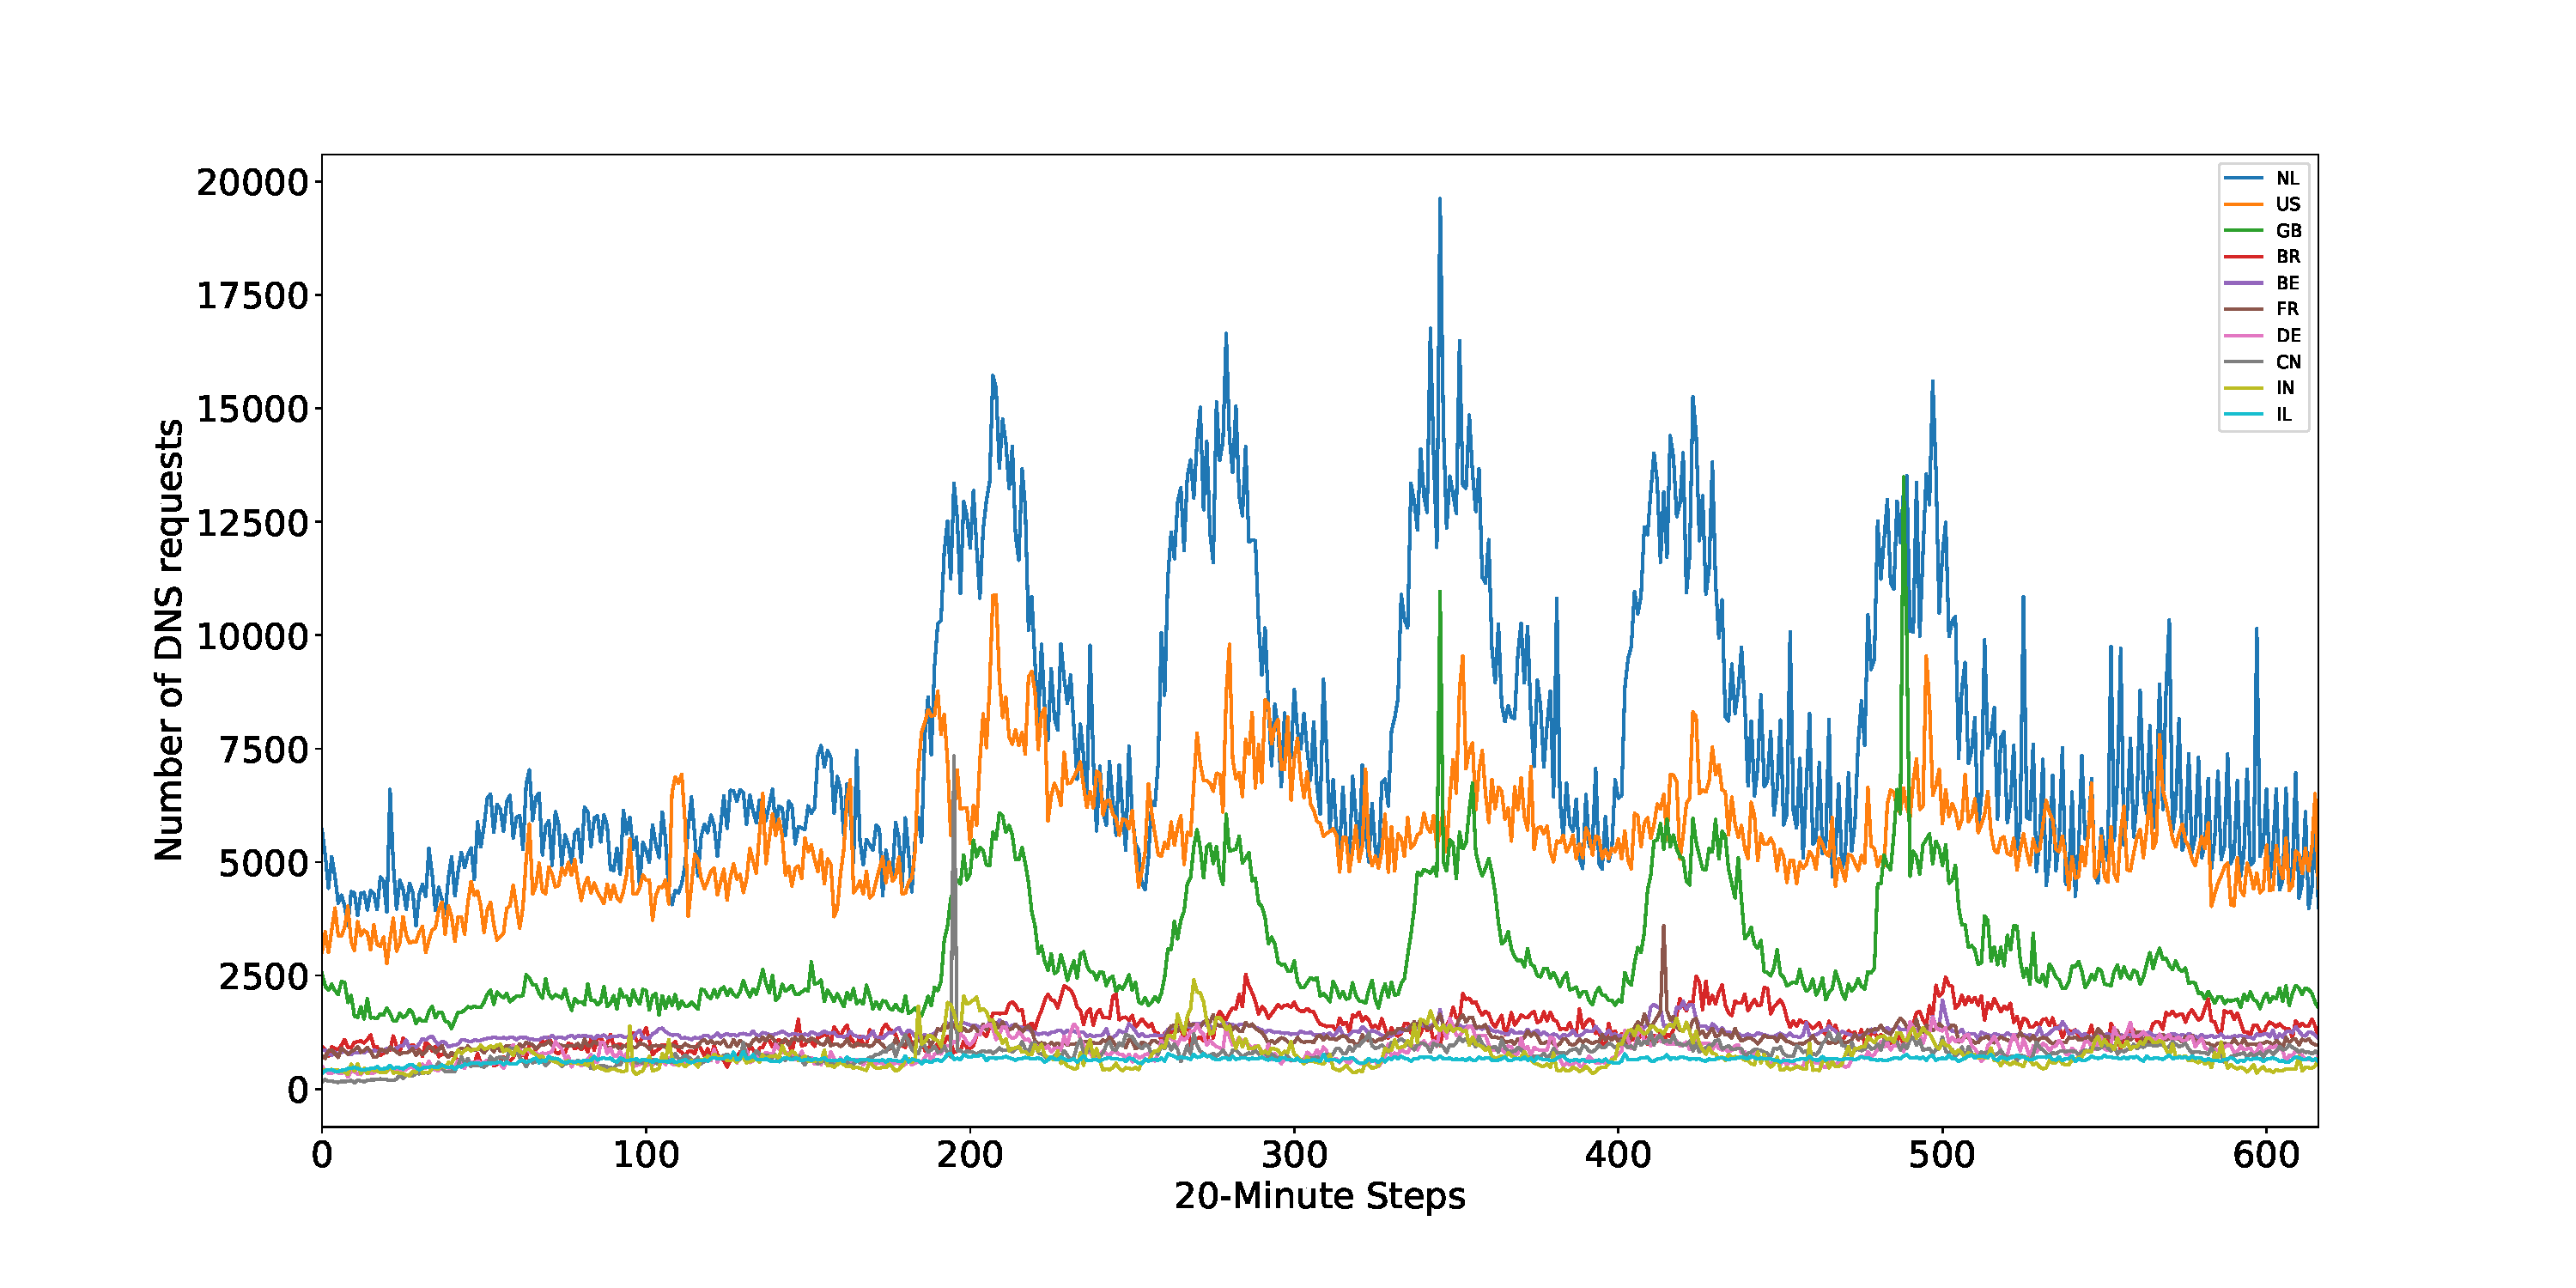
\includegraphics[width=1\linewidth]{Pictures/Dataset/GoogleSet10CountriesFirstWeek}
	\caption{Plot of the data in the Google set. Combined into 20-minute steps displayed are only the first ca. 600 steps with only the 10 countries with the most DNS requests.}
	\label{fig:googleset10countriesfirstweek}
\end{figure}

A similar dataset is a set from \cite{10.1007/978-3-319-95168-3_37}.
This data includes IP-packets of a university network, each packet labelled with application information. Examples include Google, HTTP or YouTube.
The plot in figure \ref{fig:kagglesetplottop9apps} shows how the data changes over time.
It also shows a problem with this set.
The recording intervals were not adjacent to one another, leading to vast stretches with no data.

\begin{figure}
	\centering
	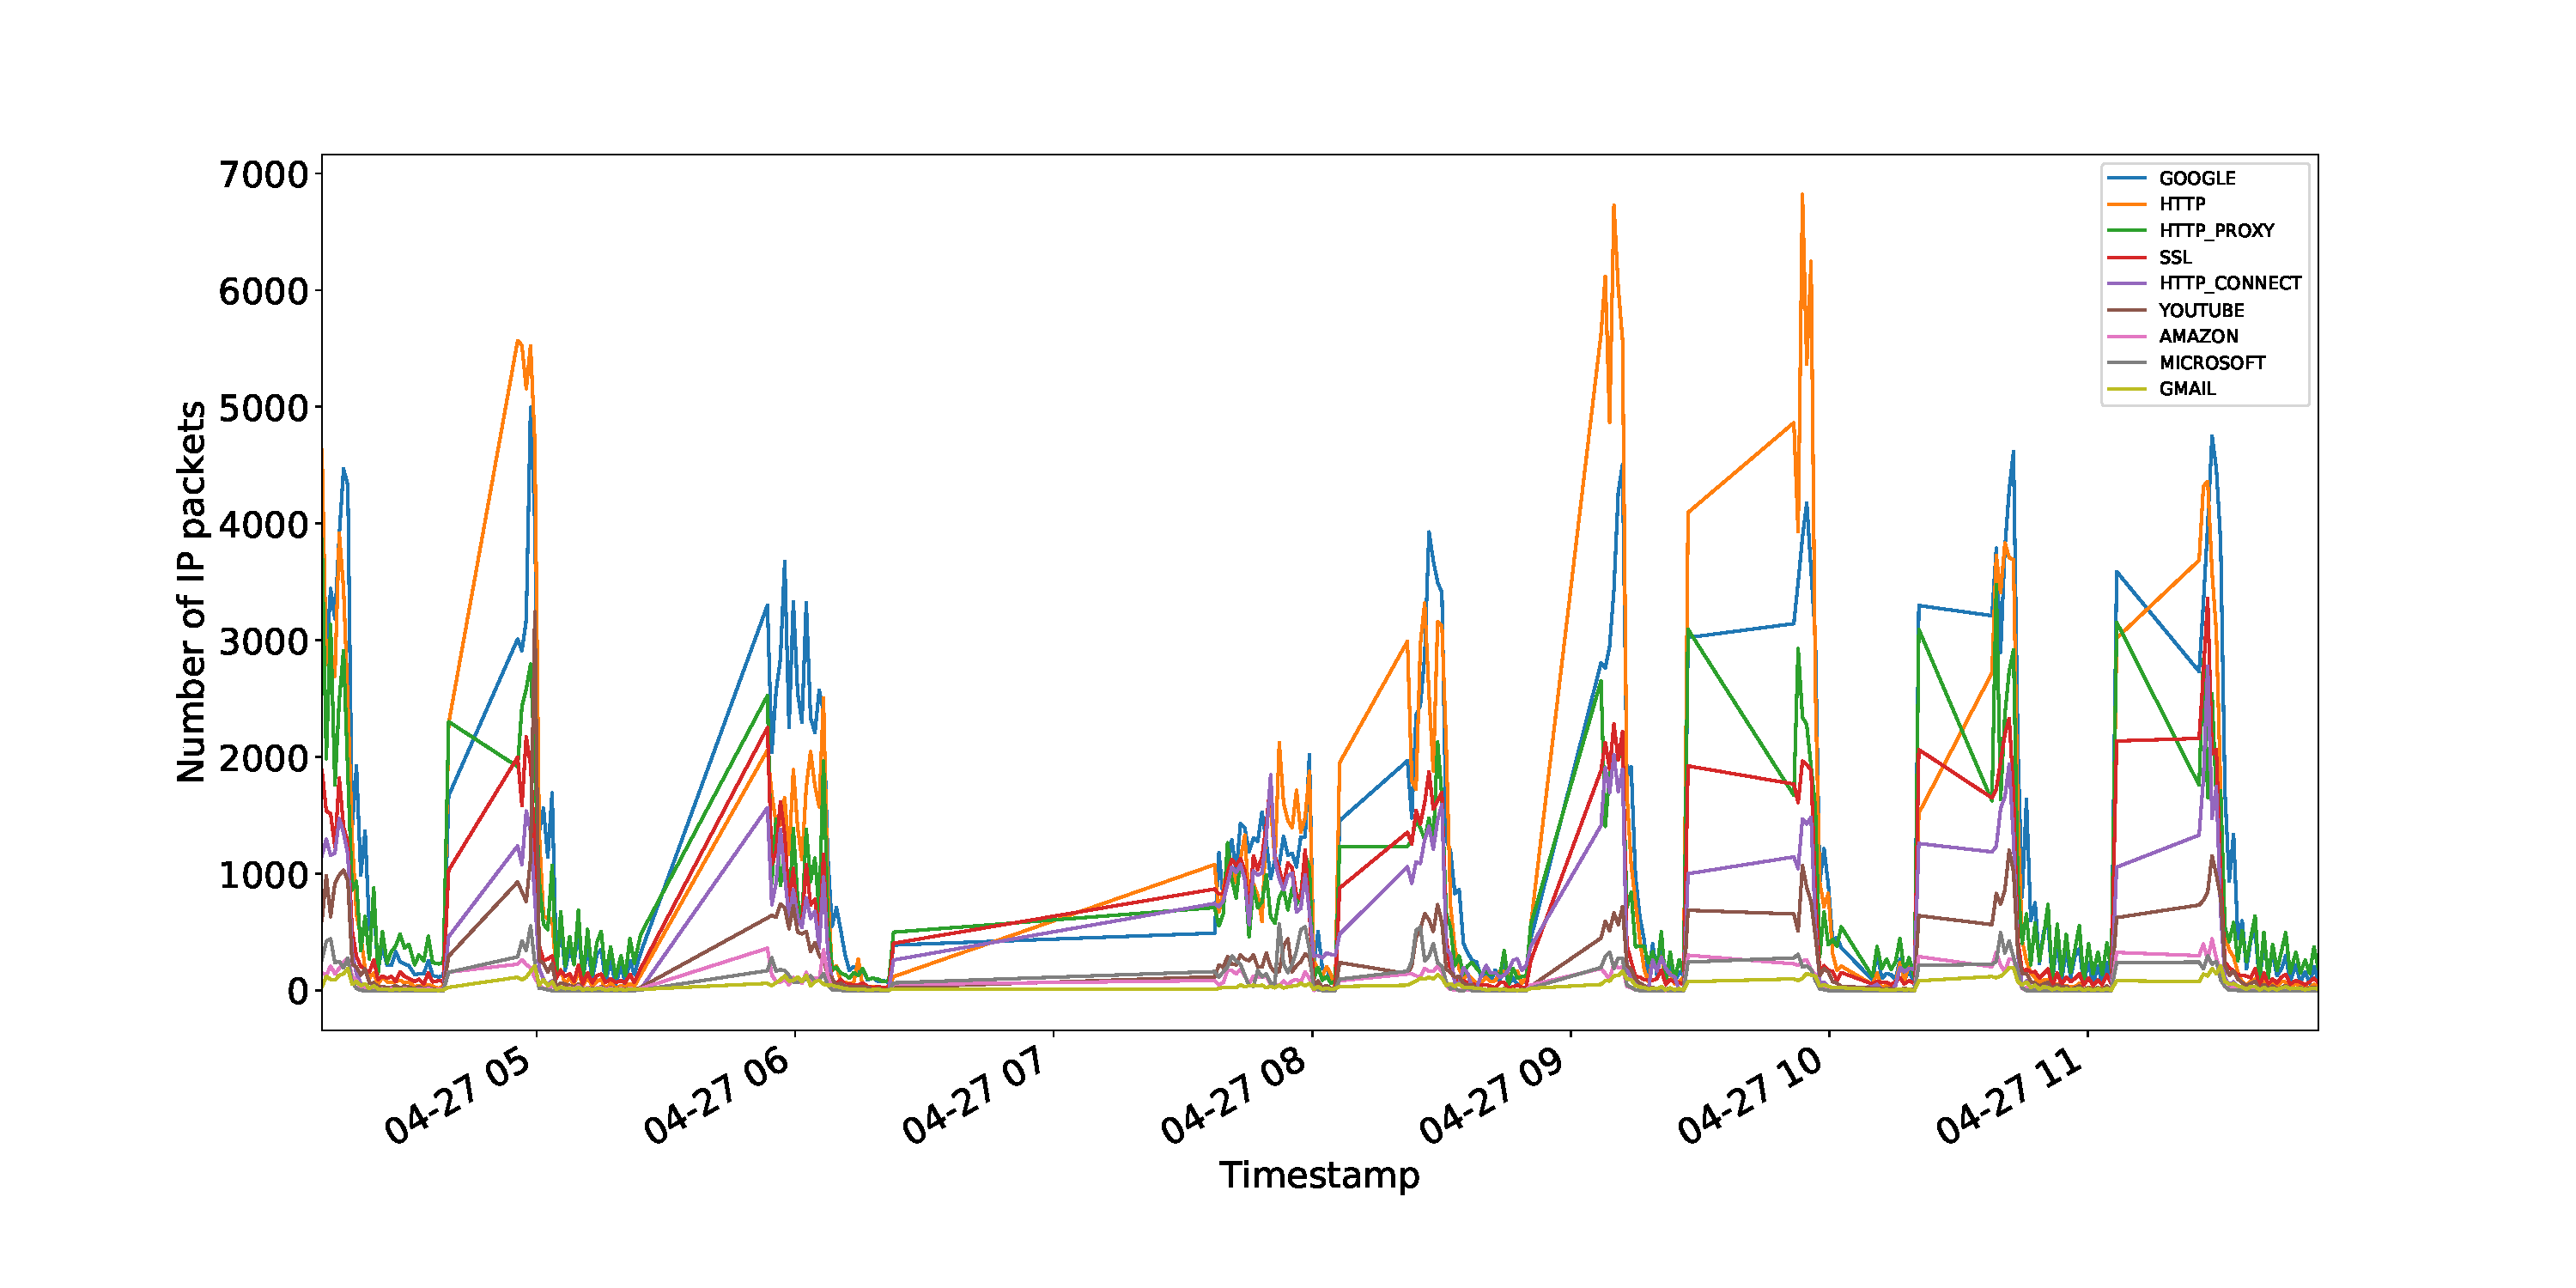
\includegraphics[width=1\linewidth]{Pictures/Dataset/KaggleSetPlotTop9Apps}
	\caption{Plot of the set from Kaggle. Included are the nine most requested apps.}
	\label{fig:kagglesetplottop9apps}
\end{figure}

A set containing another type of data is the set from \cite{SNDlib10}, \cite{OrlowskiPioroTomaszewskiWessaely2010}.
It contains the bandwidth of all pairs communicating in the network, combined into 15-minute steps.
The data originates from the GÉANT network, a European research network, including 23 nodes all over Europe.
The plot \ref{fig:totemplotfirstweek6destinationsfrom1} shows the data from the first week with the source as node 1 and destinations nodes 1 to 6.
The data was anonymized, that is why a number only denotes the nodes.
Also, the data was collected over four months.

The last data collection originates from the Abilene network in the USA from \cite{SNDlib10}, \cite{OrlowskiPioroTomaszewskiWessaely2010}.
It is in the same format as the previous dataset, but this network includes fewer nodes then the GÉANT network.
However, it has a higher accuracy with 5-minute steps and the recording ran over an extended period of 6 months.
Here an argument can be made for both datasets, depending on what is needed: more diversity in the nodes or higher accuracy.

\begin{figure}
	\centering
	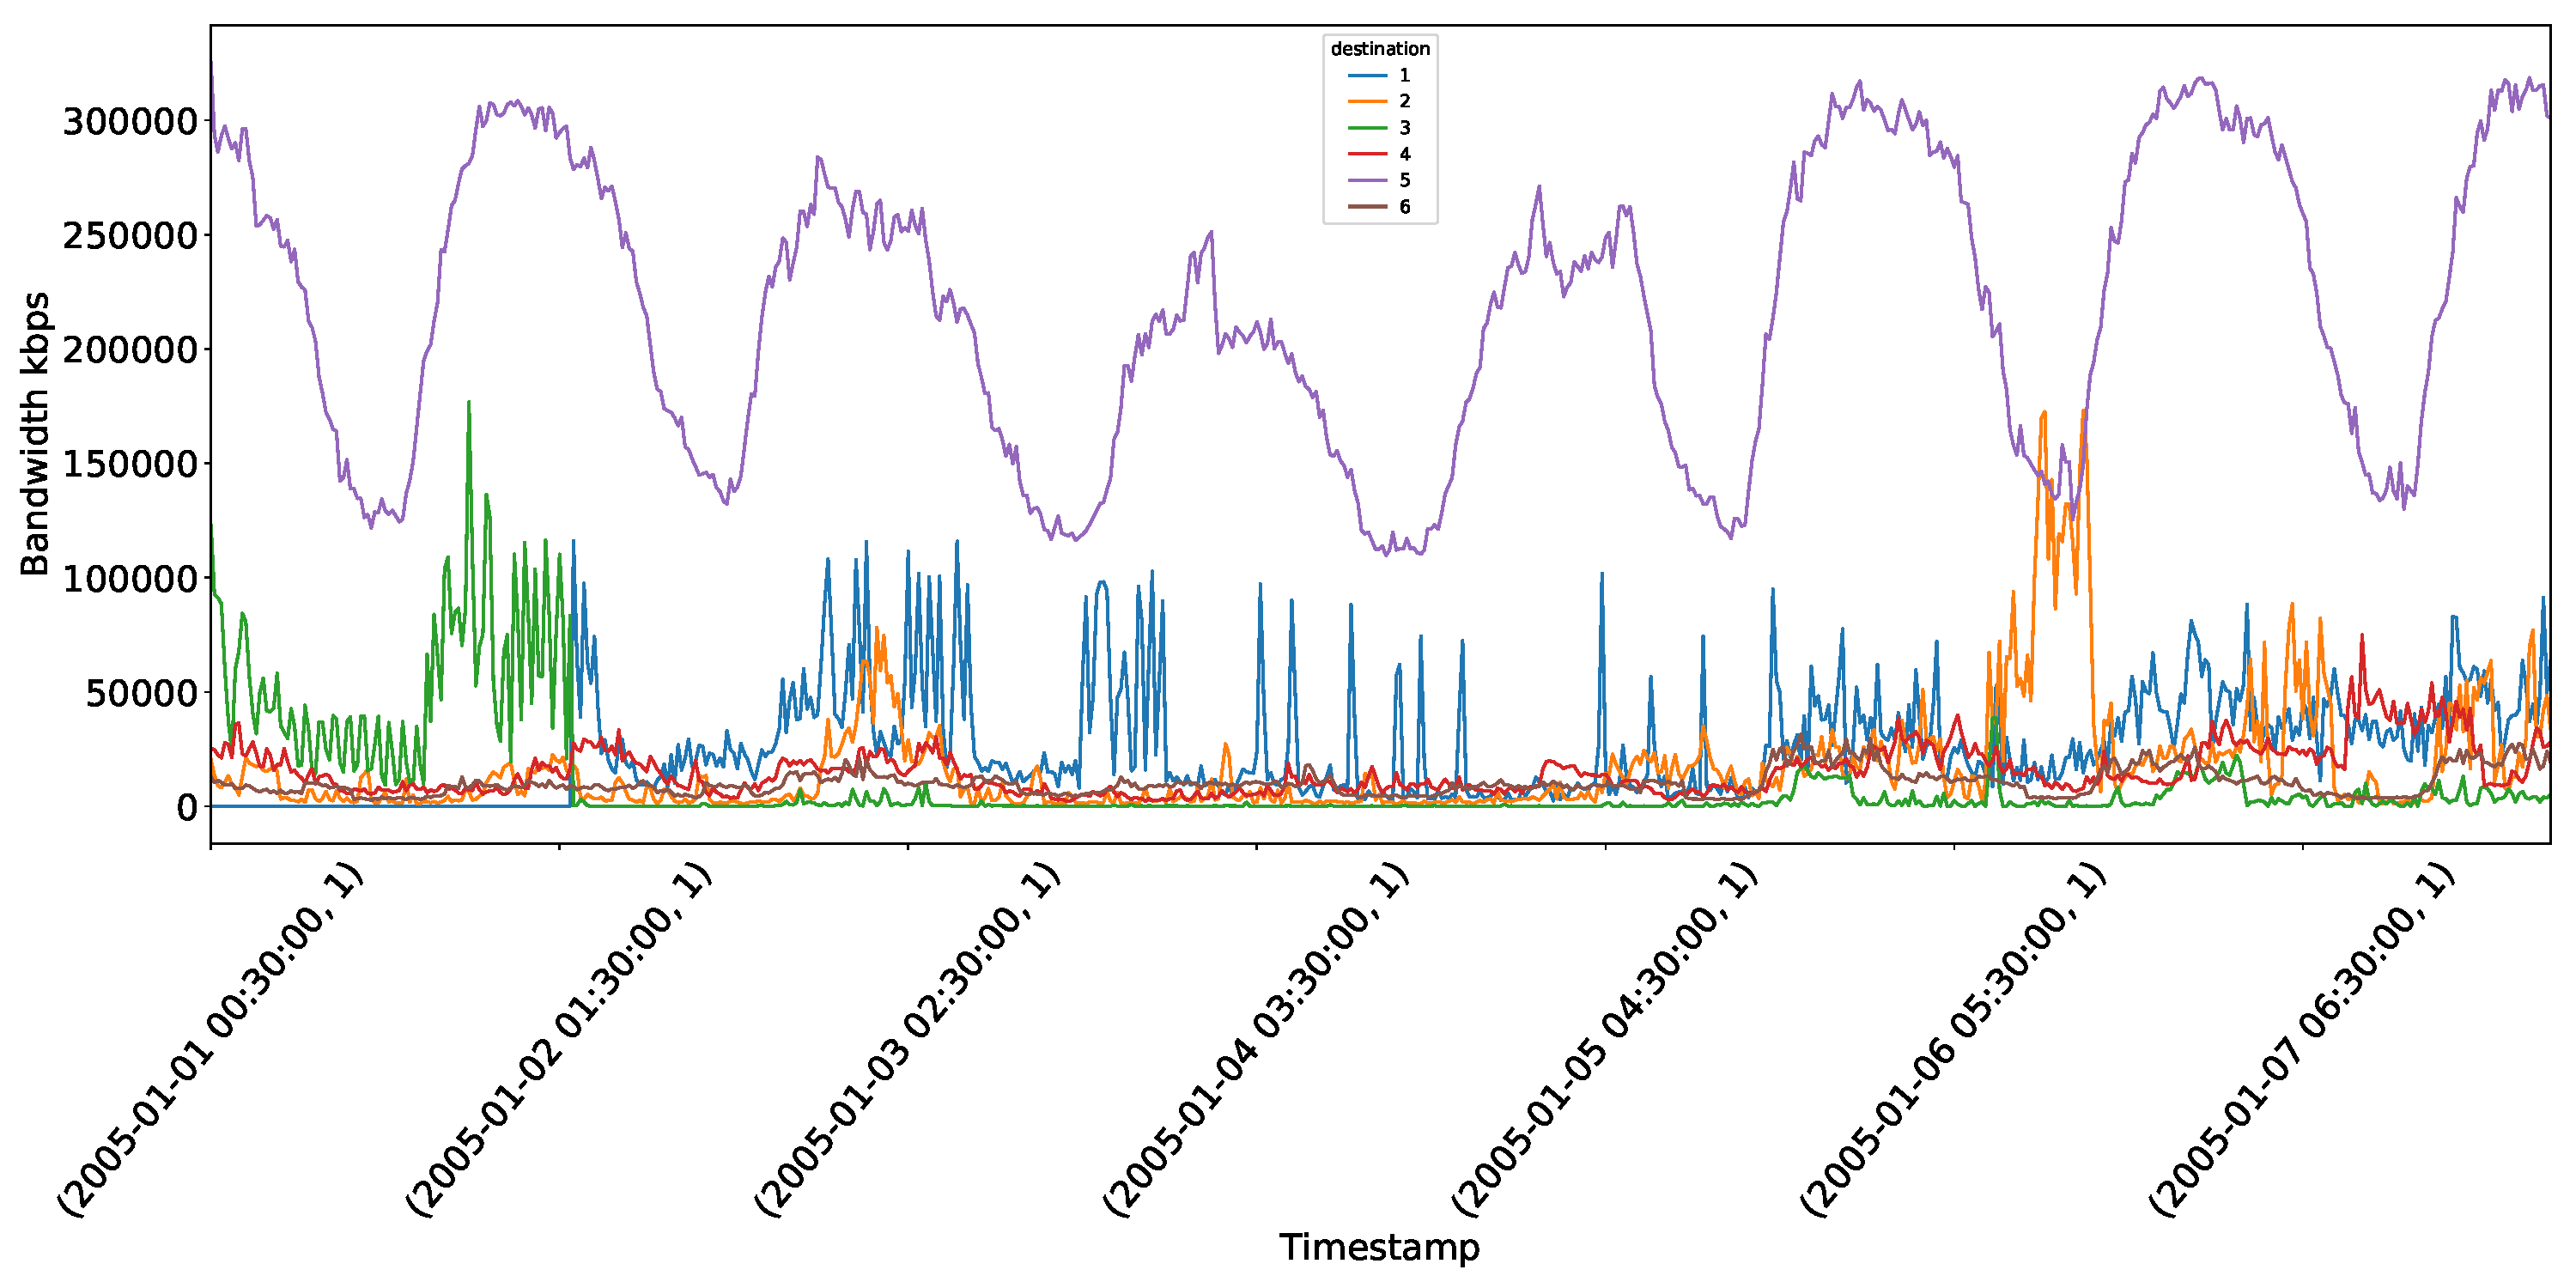
\includegraphics[width=1\linewidth]{Pictures/Dataset/TOTEMPlotFirstWeek6DestinationsFrom1}
	\caption{Plot of the network bandwidth from GÉANT network from source 1 to the first 6 destinations.}
	\label{fig:totemplotfirstweek6destinationsfrom1}
\end{figure}

\subsection{Choosing a Dataset}\label{chooseDataset}
The goal of this thesis is the prediction of the different service requests for each ingress node.
With that in mind, a dataset would be ideal that either provides the service request per ingress node or a dataset that can work as a substitution for service traffic.
Since none of the six datasets contains actual service traffic, one of the six has to substitute the service traffic.

The set from Alibaba \footnote{\url{https://github.com/alibaba/clusterdata} Accessed: 2019-11-23} and the collection from the Kaggle platform \cite{10.1007/978-3-319-95168-3_37} are both not a good fit for this application.
The Alibaba set is not representing the network traffic itself but the jobs and batches running on the machines in the network.
Maybe with much work, the traffic could be inferred from the jobs running on the machines, but that is not worth the work for this thesis when other sets are available.
The IP packet set from Kaggle, on the other hand, would represent a good substitution for service traffic.
With a reinterpretation of the apps as the services, the service traffic would be equal to the app traffic from Figure \ref{fig:kagglesetplottop9apps}.
However, the long periods where data is missing in the traffic make it not suitable for training a machine learning model.

Furthermore, the data from the knowledge defined networking dataset \cite{Mestres:2017:KN:3138808.3138810} is not the best choice for the work of this thesis.
Since the data of this set is the result of a simulation, the credibility of real-world data is missing.
Because the developed models should be trained with real-world data to get realistic results, I will not use this data.

The DNS requests in the Google dataset \cite{8506536} are a better fit at the first look.
It is a highly detailed dataset; each DNS request is recorded and fitted with a timestamp.
However, since these records are DNS requests, it would not be the best idea to develop models that predict network service traffic, since network service traffic is behaving differently than DNS traffic.
Also, what is missing are ingress nodes, that would lead to much reinterpretation and modification of the data, which would decrease the credibility of the results.

The two last sets are the GÉANT network data and the Abilene set \cite{SNDlib10}, \cite{OrlowskiPioroTomaszewskiWessaely2010}.
Both represent real network traffic between nodes and contain the traffic of all pairs in the network.
Both datasets also span many months.
So there is much variety to choose from with traffic at weekends, workweek traffic and also traffic at bank holidays.
In the end, the choice fell on the GÉANT network data because of the more substantial number of nodes and the resulting diversity.

\subsection{Modifications of the Dataset}\label{datasetMod}
After choosing the dataset, the task is to interpret and add to the data so that a model can be trained that predicts service network traffic.
When looking at the GÉANT network, the data contains all pairs and their bandwidth in 15-minute steps.
So for the model, a network $N = (V,L)$ is needed where each service traffic $x_{n}$ can be defined to each ingress node $I\in V$.
This requirement needs to be applied to the GÉANT network data and can be fulfilled when taking a subset of the nodes and looking at the traffic of the pairs.
The subset that was taken can be interpreted as the ingress node and the traffic going to these nodes can also be interpreted as the bandwidth for each service.
As an example, if the service subset is node 1 to 10, then the remaining nodes 11 to 23 are interpreted as the ingress nodes.
This results in a detailed record of how much bandwidth each service to each ingress node uses.
The reinterpretation also has the positive effect that I do not have to change the data.

The same assumption can be made for the Abilene set \cite{SNDlib10}, \cite{OrlowskiPioroTomaszewskiWessaely2010}.
The only difference here is the number of nodes, that leads to more diversity in the network GÉANT network; that is why I chose the GÉANT network.